%%%%%%%%%%%%%%%%%%%%%%%%%%%%%%%%%%%%%%%%%
% Beamer Presentation
% LaTeX Template
% Version 1.0 (10/11/12)
%
% This template has been downloaded from:
% http://www.LaTeXTemplates.com
%
% License:
% CC BY-NC-SA 3.0 (http://creativecommons.org/licenses/by-nc-sa/3.0/)
%
%%%%%%%%%%%%%%%%%%%%%%%%%%%%%%%%%%%%%%%%%

%----------------------------------------------------------------------------------------
%	PACKAGES AND THEMES
%----------------------------------------------------------------------------------------

\documentclass[aspectratio=169]{beamer}

\mode<presentation> {

% The Beamer class comes with a number of default slide themes
% which change the colors and layouts of slides. Below this is a list
% of all the themes, uncomment each in turn to see what they look like.

%\usetheme{default}
%\usetheme{AnnArbor}
%\usetheme{Antibes}
%\usetheme{Bergen}
%\usetheme{Berkeley}
%\usetheme{Berlin}
%\usetheme{Boadilla} %maybe
%\usetheme{CambridgeUS}
%\usetheme{Copenhagen}
%\usetheme{Darmstadt}
%\usetheme{Dresden}
%\usetheme{Frankfurt}
%\usetheme{Goettingen}
%\usetheme{Hannover}
%\usetheme{Ilmenau}
%\usetheme{JuanLesPins}
%\usetheme{Luebeck}
%\usetheme{Madrid} %maybe
%\usetheme{Malmoe}
%\usetheme{Marburg}
%\usetheme{Montpellier}
%\usetheme{PaloAlto}
%\usetheme{Pittsburgh}
%\usetheme{Rochester}
%\usetheme{Singapore}
%\usetheme{Szeged}
%\usetheme{Warsaw}

\usetheme{metropolis}

% As well as themes, the Beamer class has a number of color themes
% for any slide theme. Uncomment each of these in turn to see how it
% changes the colors of your current slide theme.

%\usecolortheme{albatross}
%\usecolortheme{beaver}
%\usecolortheme{beetle}
%\usecolortheme{crane}
%\usecolortheme{dolphin}
%\usecolortheme{dove}
%\usecolortheme{fly}
%\usecolortheme{lily}
%\usecolortheme{orchid}
%\usecolortheme{rose}
%\usecolortheme{seagull}
%\usecolortheme{seahorse}
%\usecolortheme{whale}
%\usecolortheme{wolverine}

%\setbeamertemplate{footline} % To remove the footer line in all slides uncomment this line
%\setbeamertemplate{footline}[page number] % To replace the footer line in all slides with a simple slide count uncomment this line

%\setbeamertemplate{navigation symbols}{} % To remove the navigation symbols from the bottom of all slides uncomment this line
}

\usepackage{graphicx} % Allows including images
\usepackage{booktabs} % Allows the use of \toprule, \midrule and \bottomrule in tables
\usepackage{multirow}
\usepackage{multicol}
\usepackage{graphics}
\usepackage{ bbold }
\setbeamersize{text margin left=15pt,text margin right=15pt}

%----------------------------------------------------------------------------------------
%	TITLE PAGE
%----------------------------------------------------------------------------------------

\title{Deep Learning on Kubeflow}  
\subtitle{}
\author{Iurii Mozzhorin, Rebekka Pech}
\institute[Goethe University Frankfurt]{Hands-on Lab - Big Data Technologies SS 2019 \\ Goethe University Frankfurt am Main}

%\date{\today} % Date, can be changed to a custom date

\begin{document}

\begin{frame}
\titlepage % Print the title page as the first slide
\end{frame}



%----------------------------------------------------------------------------------------
%	PRESENTATION SLIDES
%----------------------------------------------------------------------------------------

%------------------------------------------------
%\section{MLBench}
%------------------------------------------------



\begin{frame}
\frametitle{What is Kubeflow?}
\begin{multicols*}{2}
\begin{itemize}
	\item an open-source platform 
	\item based on Kubernetes 
	\item simple, portable and scalable deployments of ML 
	\item integration of existing tools and libraries
\end{itemize}

\begin{block}{Includes components for}
	\begin{itemize}
		\item model developing, training, serving
		\item hyperparameter tuning
		\item pipelines
	\end{itemize}
\end{block}
\pagebreak
\begin{figure}
	
\includegraphics[width=0.25\textwidth]{kubeflowlogo.png}
\end{figure}
\end{multicols*}
\end{frame}

%------------------------------------------------

\begin{frame}
\frametitle{Use case}

\begin{block}{Goal}
	\begin{itemize}
		\item \large Train a CNN model to distinguish between works of 10 painters
	\end{itemize}
\end{block}

\begin{block}{Dataset}
	\begin{multicols*}{2}
	\begin{itemize}
		\item "Painter by Numbers" from Kaggle.com
		\item Original size 83GB
		\item Images dimensions $477 - 7444$ px
		\item Selected \& resized: 
		\begin{itemize}
			\item 340 MB
			\item 388 images $\times$ 10 artists
			\item images smallest dimension 448 px 
		\end{itemize}
		\item Test set 20 images (5\%)
	\end{itemize}
	\begin{figure}
		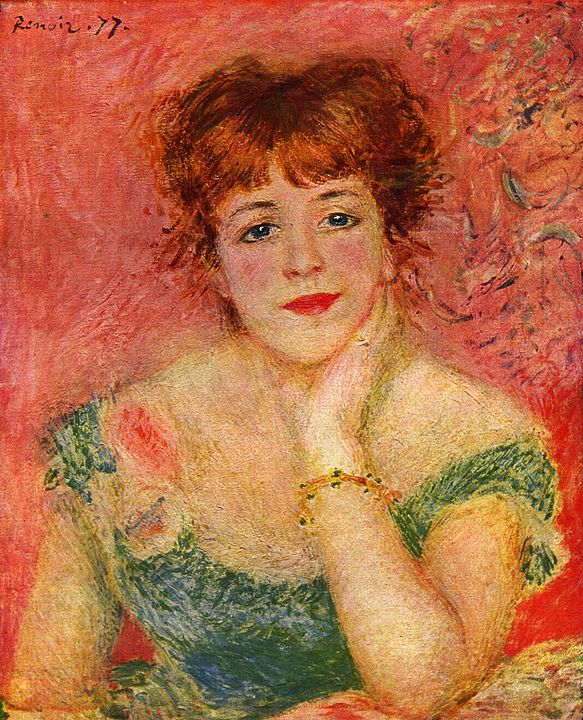
\includegraphics[width=0.25\textwidth]{Renoir}
	\end{figure}

	\end{multicols*}
\end{block}

\end{frame}

%------------------------------------------------

\begin{frame}
\frametitle{Use case}

\begin{block}{Model}
	\begin{itemize}
		\item ResNet 50
		\item Transfer learning with weights from ImageNet (1000 classes)
		\item Input size $224 \times 224$ px
		\item Image augmentation: shift, rotation, flip
	\end{itemize}
\end{block}
\begin{figure}
	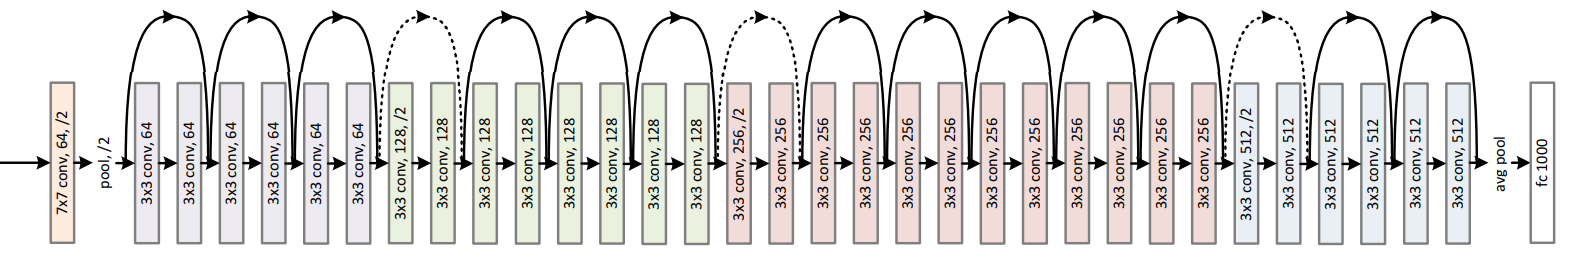
\includegraphics[width=1\textwidth]{resnet}
\end{figure}

\end{frame}


%------------------------------------------------

\begin{frame}
\frametitle{Tasks/Milestones}

\begin{itemize}
	\item Preprocess the data
	\item Create the model (transfer learning)\\
	\item Create the Docker image\\
	\item Train the model on KF using TFJobs on CPUs\\
	\item Save the trained model\\
	\item Train the model on KF using TFJobs on GPUs\\
	\item Distributed training on multiple pods\\
	\item Serve the model
\end{itemize}

\end{frame}

%------------------------------------------------

\begin{frame}
\frametitle{Technologies}

\begin{itemize}
	\item Create the model: TF $\rightarrow$ Keras
	\item Containers: Docker and Kubernetes
	\item Manage pods (TFJobs): kubectl + ksonnet $\rightarrow$ kubectl + kustomize $\rightarrow$ kubectl
	\item Manage KF deployment: GCP console, gcloud + gsutil
	\item Manage data: PVC $\rightarrow$ GCS bucket
	\item Monitoring: Tensorboard
	\item Manage the model: TF Serving $\rightarrow$ Jupyter Notebook
\end{itemize}

\end{frame}

%------------------------------------------------

\begin{frame}
\frametitle{Analysis \& reflexion}

\begin{itemize}
	\item \textbf{Keras} simplifies work with CNN models but have several restrictions:
	\begin{itemize}
		\item cannot work directly with GCS bucket
		\item does not (directly) support distributed learning
	\end{itemize}
	\item \textbf{Tensorflow} requires additional learning time
	\item \textbf{Kubeflow} is very raw
	\begin{itemize}
		\item rapid changes, low backward compatibility
		\item requires learning of all underlying technologies 
	\end{itemize}
	\item $\Rightarrow$ \textbf{Kubeflow does not suit for research in data science} 
\end{itemize}

\end{frame}

%------------------------------------------------

\begin{frame}
\frametitle{References}

\begin{itemize}
	\item https://www.kubeflow.org/docs/
	\item https://github.com/kubeflow/examples
	\item https://www.kaggle.com/c/painter-by-numbers/
	\item Kaiming He, Xiangyu Zhang, Shaoqing Ren, Jian Sun. Deep Residual Learning for Image Recognition, arXiv:1512.03385
	\item https://keras.io/
	\item https://www.tensorflow.org/guide
	\item https://kubernetes.io/docs/
	
\end{itemize}

\end{frame}

%------------------------------------------------

\begin{frame}
\Huge{\centerline{Thank you for your attention!}}\end{frame}





\end{document} 